%--------------------------------------------------------
%--------------------------------------------------------
%\section{The spin-0 description of CMB polarization} \label{sec:pol-intro}
%--------------------------------------------------------
\section{Polarization primer}\label{sec:pol-primer}
The CMB polarization is measured in terms of Stokes Q and U parameters. These measurements can be combined to form the complex spin 2 polarization field as follows,
%
\beqry \label{eq:spin-pol}
_{\pm 2}\bar{X}(\hat{n}) &=& Q(\hat{n}) \pm i U (\hat{n}) \nonumber \\ &=& \sum_{\ell m}  {_{\pm 2}} \tilde{X}_{\ell m}  \, {_{\pm 2}}Y_{\ell m} (\hat{n}) \,.
\eeqry
%
Since these measured quantities depend on the local coordinate system, it is cumbersome to work with them. To overcome this, one describes the CMB polarization field in terms of a scalar field denoted by $E(\hat{n}) $ and a pseudo scalar field $B(\hat{n}) $ \cite{Kamionkowski1997}. These scalar fields are related to the spin-2 polarization field $_{\pm 2}X(\hat{n})$ via the following relations,
%
\beq \label{eq:ebdef}
\mathcal{E}(\hat{n}) = -\frac{1}{2} \big[ \bar{\eth}^2 _{+ 2}\bar{X}(\hat{n})  +  \eth^2 _{- 2}\bar{X}(\hat{n}) \big] ~\,;~\mathcal{B}(\hat{n}) = -\frac{1}{2i} \big[ \bar{\eth}^2 _{+ 2}X(\hat{n})  -  \eth^2 _{- 2}X(\hat{n}) \big] \,,
\eeq
%
where $\eth$ and $\bar{\eth}$ denote the spin raising and lowering operators respectively. These $E$ and $B$ fields are spin-0 fields similar to the temperature anisotropies and hence their value are independent of the coordinate system definitions (except that the B-modes have an odd parity, meaning that they change sign under reflection $\hat{n} \rightarrow -\hat{n}$.). The spin raising and lowering operators have the following properties \cite{goldberg67},
%
\beqrys \label{eq:spinopylm} 
\eth _s Y_{lm}(\hat{n}) &=& \sqrt{(\ell-s)(\ell+s+1)} _{s+1} Y_{lm}(\hat{n}) \,, \\
\bar{\eth} _s Y_{lm}(\hat{n}) &=& -\sqrt{(\ell+s)(\ell-s+1)} _{s-1} Y_{lm}(\hat{n}) \,, 
\eeqrys
%
where $_s Y_{lm}(\hat{n}) $ denote the spin-s spherical harmonics.

Using \eq{eq:ebdef} and the properties of the spin raising and lowering operators given in \eq{eq:spinopylm} it can be shown that the scalar fields $\mathcal{E}/\mathcal{B}$ are defined via the following set of equations,
%
\beq \label{eq:pseudo}
\mathcal{E}(\hat{n}) = \sum_{\ell m} a^{E}_{\ell m} \sqrt{\frac{(\ell+2)!}{(\ell-2)!}} Y_{\ell m} (\hat{n}) ~\,;~ \mathcal{B}(\hat{n})  =\sum_{\ell m} a^{B}_{\ell m} \sqrt{\frac{(\ell+2)!}{(\ell-2)!}} Y_{\ell m} (\hat{n}) \,,
\eeq
%
where the harmonic coefficients of  $\mathcal{E}/\mathcal{B}$ fields are related to the harmonic coefficients of the spin-2 polarization field via the following equations,
%
\beq\label{eq:x2eb}
a^{E}_{\ell m} = -\frac{1}{2} \Big[ {}_{+2}\tilde{X}_{\ell m} + {}_{-2}\tilde{X}_{\ell m} \Big] ~\,;~a^{B}_{\ell m} = -\frac{1}{2i} \Big[ {}_{+2}\tilde{X}_{\ell m} - {}_{-2}\tilde{X}_{\ell m} \Big] 
\eeq
%
In the remainder of this article, we will work with the scalar $E$ and pseudo scalar $B$ fields as defined by the following expressions, 
%
\beq \label{eq:realeb}
E(\hat{n}) = \sum_{\ell m} a^{E}_{\ell m} Y_{\ell m} (\hat{n}) ~\,;~ B(\hat{n})  =\sum_{\ell m} a^{B}_{\ell m} Y_{\ell m} (\hat{n}) \,.
\eeq
%
Note that the $[E,B]$ fields are merely filtered versions of the fields $[\mathcal{E},\mathcal{B}]$, as their spherical harmonic coefficients of expansion differ by the factor $\sqrt{\frac{(\ell+2)!}{(\ell-2)!}}$. %We make this choice since the CMB spectra are more closely related to the fields E \& B.
%--------------------------------------------------------
%--------------------------------------------------------
\subsection{Matrix notation} \label{sec:mat_pol_intro}
In this section we cast the relations introduced in Sec.~\ref{sec:pol-primer} in matrix notation\footnote{While we work with the matrix and vector sizes given in terms of some pixelization parameter $\rm N_{\rm pix}$, all the relations are equally valid in the continuum limit attained by allowing $\rm N_{\rm pix}\rightarrow \infty$}. This representation will make transparent the derivation of the real space operators we discuss in the following sections. We adopt a convention in which real space quantities are denoted by bar-ed variable while those in harmonic space are denoted by tilde-ed variables.

We begin by introducing the matrices encoding the spin spherical harmonic basis vectors,
%
\beq
{}_{|s|}\mathcal{Y}= \bmat _{+s}Y & 0 \\ 0 & _{-s}Y \emat _{2 \rm N_{\rm pix} \times 2 \rm N_{\rm alms}} \,,
\eeq
%
where $s$ denotes the spin of the basis functions. For this work we will be working with cases $s \in [0,2]$. In this notation, each column can be mapped to a specific harmonic basis function marked by the pair of indices: $(\ell,m)$ and each row maps to a specific position on the sphere. Note that this matrix is in general not a square matrix. The number of rows is determined by the scheme used to discretely represent the sphere and the number of columns is set by the number of basis functions of interest (often determined by the band limit).

We now define the different polarization data vectors and their representation in real and harmonic space as follows,
%
\beqrys
\bar{S} &=& \bmat E \\ B  \emat_{2 \rm N_{\rm pix} \times 1} ~~~~;~~ \bar{X} = \bmat _{+2}X \\ _{-2}X \emat_{2 \rm N_{\rm pix} \times 1} ~~;~~\bar{P} =\fqu_{\tiny {2 \rm N_{\rm pix} \times 1}} \,, \\
\tilde{S} &=& \bmat a^{E} \\ a^{B} \emat _{2 \rm N_{\rm alms} \times 1}  ~~; ~~ \tilde{X} = \bmat _{+2} \tilde{X} \\ _{-2} \tilde{X} \emat_{2 \rm N_{\rm alms} \times 1} \,.
\eeqrys
%
The different symbols have the same meaning as that discussed in \sec{sec:pol-primer}, except that the subscript $_{\ell m}$ for the spherical harmonic coefficients of expansion is suppressed if favor of cleaner notation.

Next we define the operators which govern the transformations between different representations of the polarization field as follows,
%
\beqrys
\bar T &=& \qutox_{2 \rm N_{\rm pix} \times 2 \rm N_{\rm pix}} ~~;~~ \bar T^{-1} = \frac{1}{2} \bar T^{\dagger} \,, \\
\tilde T &=& -\qutox_{2 \rm N_{\rm alms} \times 2 \rm N_{\rm alms}} ~~;~~ \tilde T^{-1} = \frac{1}{2} \tilde T^{\dagger} \,,
\eeqrys
%
where we have chosen the sign conventions so as to match those used in Healpix.
Using the data vectors and the matrix operators defined above we can now express, in compact notation, the forward and inverse relations between different representations of the polarization data vectors as follows,
%
\begin{subequations} \label{eq:pol_data_relns}
\beqry 
\bar{X} &=& \bar T * \bar{P} ~~;~~\bar{P} = \frac{1}{2} \bar T^{\dagger} * \bar{X} \,, \\
\bar X &=&  {{}_2\mathcal{Y}} * \tilde X  ~~;~~ \tilde X ={{}_2\mathcal{Y}}^{\dagger} * \bar X  \,, \\
\tilde{X} &=& \tilde T * \tilde{S} ~~;~~ \tilde{S} = \frac{1}{2}\tilde T^{\dagger} * \tilde{X} \,.\\ 
\bar S &=&  {{}_0\mathcal{Y}} * \tilde S ~~;~~  \tilde S =  {{}_0\mathcal{Y}}^{\dagger} * \bar S \,.
%\tilde X &=&  {{}_2\mathcal{Y}}^{\dagger} * \bar X ~~;~~ \tilde{X} = \tilde T * \tilde{S} \,, \\
%\bar{S} &=& {{}_0\mathcal{Y}}*\tilde S ~~;~~ \tilde{S} = \frac{1}{2}\tilde T^{\dagger} * \tilde{X} \,.\\
%\bar{X} &=& \bar T * \bar{P} ~~;~~ \tilde{X} = \tilde T * \tilde{S} \,, \\
%\bar{P} &=& \frac{1}{2} \bar T^{\dagger} * \bar{X} ~~;~~ \tilde{S} = \frac{1}{2}\tilde T^{\dagger} * \tilde{X} \,. \\
\eeqry
\end{subequations}
%
Next we introduce the harmonic space operators, which project the harmonic space data vector to E or B subspace,
%
\begin{subequations} \label{eq:har_eb_op}
\beqry
\tilde O_E &=& \bmat \mathbb{1} & \mathbb{0} \\ \mathbb{0} & \mathbb{0} \emat _{2 \rm N_{\rm alms} \times 2 \rm N_{\rm alms} }   ~~;~~ \tilde S_E = \tilde O_E* \tilde S \,,\\
\tilde O_B &=& \bmat \mathbb{0} & \mathbb{0} \\ \mathbb{0} & \mathbb{1} \emat _{2 \rm N_{\rm alms} \times 2 \rm N_{\rm alms} } ~~; ~~ \tilde S_B = \tilde O_B *\tilde S \,
\eeqry
\end{subequations}
%
Note that these harmonic space matrices are idempotent, orthogonal to each other and their sum is an identity matrix as can be explicitly seen via the following relations, 
%
\begin{subequations} \label{eq:har_op_prop}
\beqry
\tilde O_E * \tilde O_E&=& \tilde O_E ~~;~~  \tilde O_B * \tilde O_B= \tilde O_B \,,\\
 \tilde O_E * \tilde O_B&=& \mathbb{0} \,, \label{eq:op_eb_ortho}\\ 
 \tilde O_E + \tilde O_B&=& \mathbb{1} \,.
\eeqry
\end{subequations}
%
Note that the above relations for these harmonic space operators are exactly valid.  In the following sections we aim to derive the real space analogues of these harmonic space operators.
%%%%%%%%%%%%%%%%%%%%%%%%%%%%%%%%%%%
\section{Real space operators} \label{sec:real_space_operators}
The vector-matrix notation introduced in  \sec{sec:mat_pol_intro} allows for concise book keeping of all the operations involved in the analysis of CMB polarization. In this section we use this notation to derive the real space operators which translate the Stokes vector \vp{}  to the vector of scalars \vs  and vice versa. This vector-matrix notation also allows us to simply derive real space operators for direct decomposition of the Stokes vector \vp{} in to a vector \vp{ E} that correspond to $E$-modes and another vector \vp{B} that corresponds to the $B$-modes of polarization, such that \vp{} = \vp{E} + \vp{B}, without ever evaluating the $E$ \& $B$ fields or their spherical harmonics. 
All the real space operators we derive are most conveniently expressed as functions of the Euler angles  $\alpha, ~\beta~\&~ \gamma$ on the sphere. Owing to this, we begin with a brief discussion on Euler angles and present visual method to think about them.
%
\begin{figure}[!hbt]
\centering
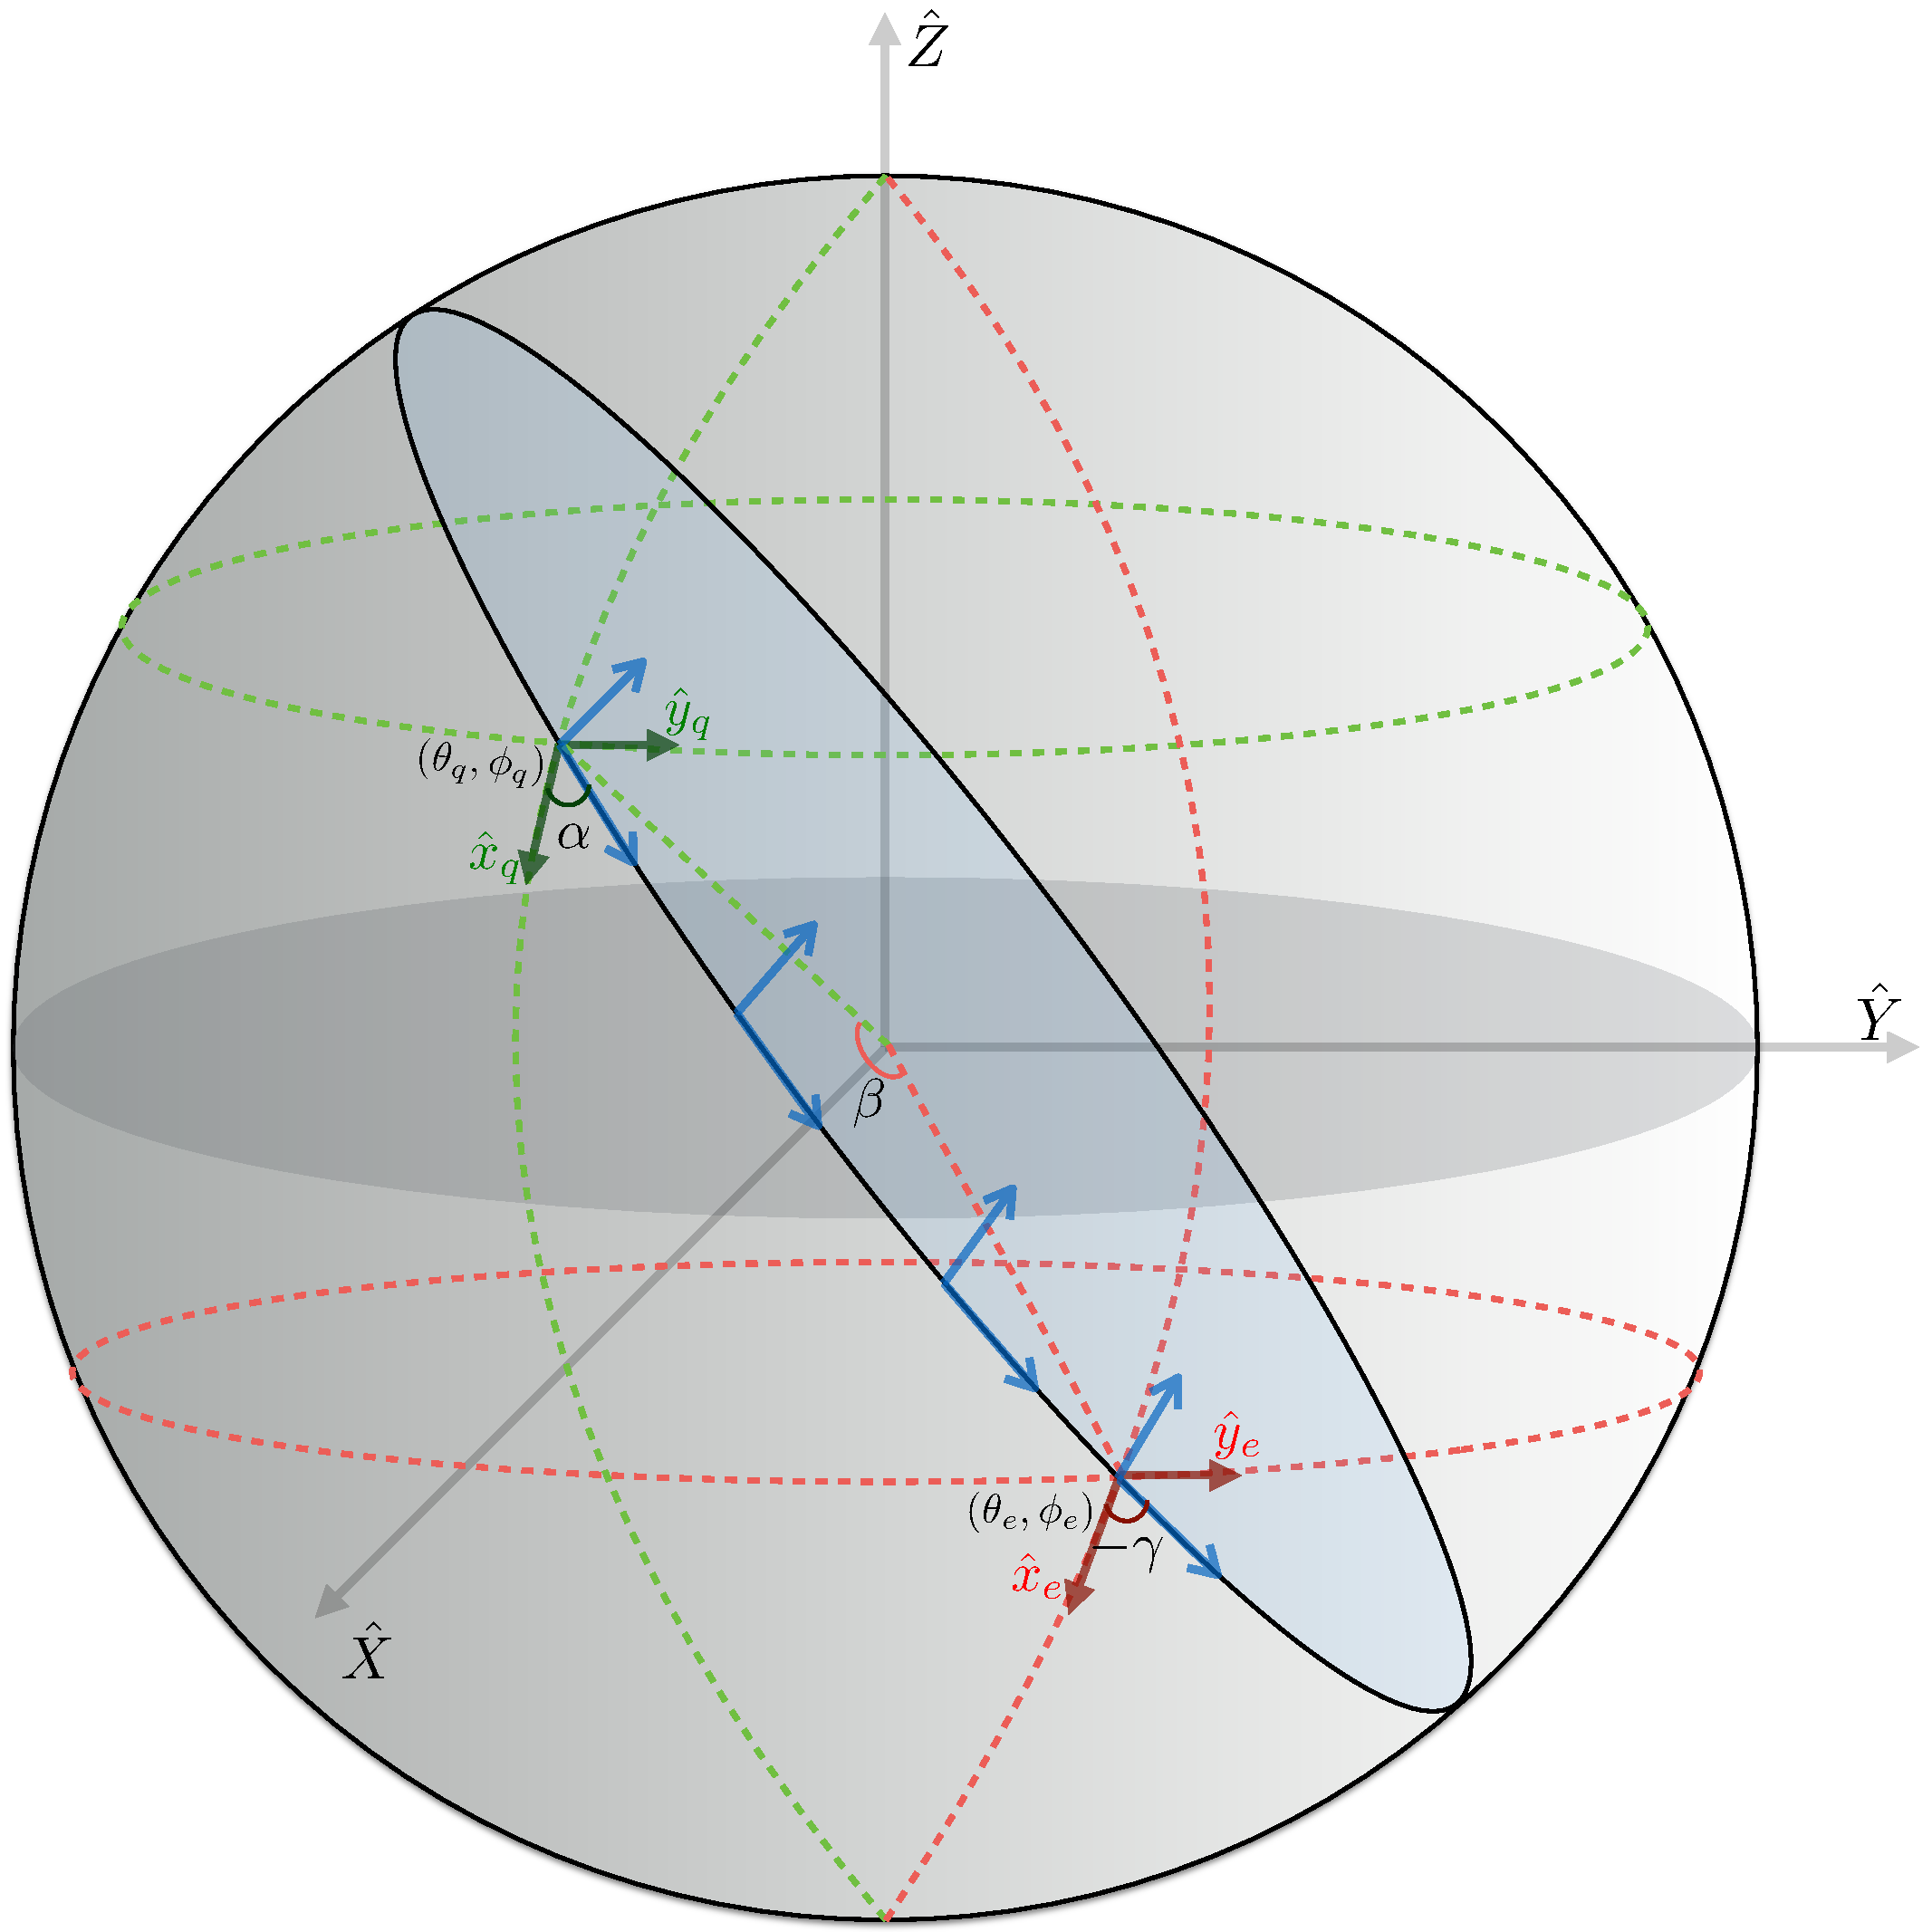
\includegraphics[width=0.5\columnwidth]{euler.pdf}
\caption{}
\label{fig:euler_angles}
\end{figure}
%
\textit{Euler angles:}  We define the local cartesian coordinate system at any point on the sphere such that the z-axis points along the radial direction, the x-axis is along the vector tangent to the local longitude pointing south and the y-axis is a vector tangent to the local latitude pointing east. The Euler angles $\alpha ,\beta ~\&~ \gamma$ define rotation operations that transforms the local cartesian coordinate system defined at the location $\hat{n}_0 \equiv (\theta_0,\phi_0)$ such that it aligns with the local cartesian coordinate system at the location $\hat{n}_i \equiv (\theta_i,\phi_i)$ \cite{varshalovich}. 

Specifically $\alpha$ defines the rotation about the z-axis, $\beta$ defines the rotation about the new y-axis (y1-axis) after the previous rotation and $\gamma$ defines the rotation about the final z-axis (z2-axis) after carrying out the previous two rotations. In more physical terms, these angles can be understood as follow: The rotation by $\alpha$ about the z-axis is such that it aligns the x-axis of the cartesian system at location $\hat{n}_0$ along the great circle in the direction of $\hat{n}_i$.  The rotation by $\beta$ about the y2-axis parallel transports the local cartesian coordinate system from location $\hat{n}_0$ to location $\hat{n}_i$, such that the z-axes of the two coordinate systems are parallel to each other. Finally the rotation by angle $\gamma$ about the z2-axis aligns the x \& y axes of the parallel transported system with those of the local cartesian system defined at $\hat{n}_i$. 

The simplest case is when one of the coordinates coincides with the north pole (more formally this refers to the point $\theta_0 \rightarrow 0$ while moving along the longitude $\phi_0=0$), say $\hat{n}_0=(\theta_0,\phi_0)=(0,0)$. In this case it is easy to visualize and infer that the rotations by Euler angles: $(\alpha,\beta,\gamma) =(\phi_i,\theta_i,0)$ in the $z-y1-z2$ sense, will align the local cartesian system at the pole with that defined at position $\hat{n}_i$. The Euler angles in the $z-y-z$ convention are related to those in the $z-y1-z2$ convection by the following rule: $(\alpha,\beta,\gamma)_{z-y-z} =(\gamma,\beta,\alpha)_{z-y1-z2}$.
%--------------------------------------------------------
\subsection{Evaluating scalar fields $E$ \& $B$ from Stokes parameters $Q$ \& $U$}\label{sec:qu2eb}
In \sec{sec:pol-primer} we described the standard procedure of computing the scalar fields E \& B from the Stokes parameters Q \& U. 
%To reiterate, this process involved taking the spin harmonic transform of the complex spin-2 fields ${}_{\pm2} \bar X$, forming specific linear combinations of the resultant coefficients of expansion ${}_{\pm 2} \tilde X_{\ell m}$ and evaluating the forward spin-0 transform to derive the scalar E \& B fields. 
Here we derive the real space convolution kernels on the sphere, which can be used to directly evaluate the scalar fields $E$ \& $B$ on the sphere.  We use the relations given in \eq{eq:pol_data_relns}, to write down an equation relating the real space vector of scalars \vs to the Stokes polarization vector \vp{},
%
\beqrys
\bar{S} &=& {{}_0\mathcal{Y}} *\tilde T^{-1}* {{}_2\mathcal{Y}^{\dagger}} *\bar T *\bar{P} = \frac{1}{2} {{}_0\mathcal{Y}} *\tilde T^{\dagger} *{{}_2\mathcal{Y}^{\dagger}} *\bar T *\bar{P}   \,, \\
&=&  \bar O *\bar{P} \,.
\eeqrys
%
The explicit form of the real space operator $\bar O$ can be derived by contracting over all the matrix operators. This procedure of contracting over the operators is explicitly worked out in the following set of equations,
%
\beqrys
\bar{O} &=& \frac{1}{2} {{}_0\mathcal{Y}} *\tilde T^{\dagger} *{{}_2\mathcal{Y}^{\dagger}} *\bar T \,, \\
&=& -0.5 \yzmat{e} \qutoxd \ymatc{q} \qutox   \,, \\
&=& -0.5 \begin{bmatrix} \sum ({}_{0}Y_e ~{}_{2}Y^{T*}_q  +  {}_{0}Y_e~ {}_{-2}Y^{T*}_q) & {\rm i}  \sum ({}_{0}Y_e ~ {}_{2}Y^{T*}_q - {}_{0}Y_e ~{}_{-2}Y^{T*}_q)  \\  - {\rm i} \sum  ({}_{0}Y_e ~ {}_{2}Y^{T*}_q - {}_{0}Y_e~ {}_{-2}Y^{T*}_q) & \sum ({}_{0}Y_e~ {}_{2}Y^{T*}_q + {}_{0}Y_e ~{}_{-2}Y^{T*}_q)  \end{bmatrix} \,, \label{eq:qu2eb_ker_1}
\eeqrys
%
where the symbol ${}_{0}Y_e$ is used to denote the sub-matrix ${}_{0}Y_{\hat{n}_e \times \ell m} \equiv {}_{0}Y_{\ell m}(\hat{n}_e)$, the symbol ${}_{\pm 2}Y^{T*}_q$ is used to denote the matrix ${}_{\pm 2}Y^*_{\ell m \times \hat{n}_q} \equiv {}_{\pm 2}Y^*_{\ell m}(\hat{n}_q)$ and the summation is over the multipole indices $\ell,m$. \revisit{We purposefully use the index ``e'' to denote the location where the scalar fields are measured and the index ``q'' to denote the location where the Stokes parameters are measured.} Using the conjugation properties of the spin spherical harmonic functions it can be shown that the following relation holds true, \comment{These constructions are dyadics}
%
\beq
 \left [\sum_{\ell m} {}_{0}Y_{\ell m}(\hat{n}_e){}_{+2}Y^*_{\ell m}(\hat{n}_q)\right]^* = \sum_{\ell m} {}_{0}Y_{\ell m}(\hat{n}_e){}_{-2}Y^*_{\ell m}(\hat{n}_q) \,.
 \eeq
 %
 where the terms on either side of the equation are those that appear in \eq{eq:qu2eb_ker_1}. The $m$ sum over the product of two spherical harmonic functions with spins $s_1$ and $s_2$ respectively, is given by the following identity \cite{varshalovich},
%
\beq \label{eq:sum_spin_shf}
 \sum_{m}{{}_{s_1}Y}^*_{\ell m}(\hat{n}_i)\,{{}_{s_2}Y}_{\ell m}(\hat{n}_j) = \sqrt{\frac{2\ell+1}{4 \pi}} {{}_{s_2}}Y_{\ell \,-s_1}(\beta_{ij},\alpha_{ij}) e^{- i s_2 \gamma_{ij}} \,,
\eeq
%
where $\alpha_{ij}, ~\beta_{ij} ~\&~ \gamma_{ij}$ denote the Euler angles. Therefore the different parts of the real space operator $\bar{O}$  are completely specified in terms of the complex function,
%
\begin{subequations}\label{eq:qu2eb_gen_kernel}
\beqry
\mathcal{M}( \hat{n}_e, \hat{n}_q)  &=& \mathcal{M}_{r} + i \mathcal{M}_{i}  \,,\nonumber \\ 
&=&\sum_{\ell m} {{_0}Y}_{\ell m}(\hat n_e) \, {{_{-2}}Y}^*_{\ell m}(\hat n_q) = \sum_{\ell} \sqrt{\frac{2\ell+1}{ 4 \pi}}{{_0Y}_{\ell 2}}(\beta_{qe},\alpha_{qe})\,,\\
&=&  \Big [ \cos(2 \alpha_{qe}) + i \sin(2 \alpha_{qe} ) \Big]   \sum_{\ell=\ell_{\rm min}}^{\ell_{\rm max}} {\frac{2\ell+1}{ 4 \pi}} \sqrt{\frac{(\ell-2)!}{(\ell+2)!}}P_{\ell 2} (\cos\beta_{qe}) \,, \label{eq:rad_ker_queb} \\
&=&  \Big [ \cos(2 \alpha_{qe}) + i \sin(2 \alpha_{qe} ) \Big] {{}_{\mm}f}(\beta_{qe},\ell_{\rm min},\ell_{\rm max}) \,, 
\eeqry
\end{subequations}
%
where we have used the identity given in \eq{eq:sum_spin_shf} to simplify the product of the spherical harmonic functions. On simplifying \eq{eq:qu2eb_ker_1}, the local convolution kernel can be cast in this simple form,
%
\beq\label{eq:op_qu2eb}
\bar O =-\bmat  \mathcal{M}_{r} & \mathcal{M}_{i} \\  -\mathcal{M}_{i}  & \mathcal{M}_{r} \emat_{2 N_{\rm pix} \times 2 N_{pix}} = -{{}_{\mm}f}(\beta_{qe},\ell_{\rm min},\ell_{\rm max})\bmat \cos(2 \alpha_{qe}) & \sin(2\alpha_{qe})\\  -\sin(2 \alpha_{qe})  & \cos(2 \alpha_{qe}) \emat \,.
\eeq
%
Specifically note that $\alpha_{qe}, ~\beta_{qe} ~\&~ \gamma_{qe}$ denote the Euler angles which rotate the local cartesian system at the location $\hat{n}_q$ where the Stokes field is measured to the cartesian system at the location $\hat{n}_e$ where the scalar fields are evaluated: $\hat{n}_q \xrightarrow{\mathcal{R}(\alpha_{qe},\beta_{qe},\gamma_{qe})} \hat{n}_e$. The Euler angles for the inverse rotations are given by the Euler angles $\alpha_{eq}=-\gamma_{qe}$, $\beta_{eq} = -\beta_{qe}$ and  $\gamma_{eq} =-\alpha_{qe}$\cite{varshalovich}. Since the kernels only depend on the cosine of the Euler angle $\beta$, they are immune to the change in its sign. More importantly, the ordering of indices  on the Euler angle $\alpha$ and $\gamma$  is important and leads to two different interpretations of the real space kernels.

\textit{Convolution:} Working from the frame of the pixel ``e'' where the scalar modes need to be evaluated, the Euler angles to the surrounding pixels are: $\alpha_{eq}, \beta_{eq},\gamma_{eq}$. In terms of these Euler angles, the value of scalar fields $E$ \& $B$ at the central pixel ``e" can be evaluated by convolving over the measured Stokes $Q$ \& $U$ parameters in the surrounding pixels marked by indices ``q''. Specifically, the convolution is fully defined in terms of the Euler angles $\beta_{eq}~ \& ~\gamma_{eq}$ and is given by the following equation,
%
\beq \label{eq:qu2eb_convolution_explicit}
\bmat E_e \\ B_e  \emat =- \sum_{q=1}^{N_{\rm pix}}{{}_{\mm}f}(\beta_{eq},\ell_{\rm min},\ell_{\rm max})\bmat \cos(2 \gamma_{eq}) & -\sin(2\gamma_{eq})\\  \sin(2 \gamma_{eq})  & \cos(2 \gamma_{eq}) \emat  \bmat Q_q \\ U_q  \emat \Delta \Omega\,,
\eeq
%
where $\Delta \Omega$ denotes the pixel area and all the symbols have their usual meaning. 
%\revisit{This has an elegant interpretation: to derive the E and/or B field at any given position we need to find the cosine quadrupole transform and the sine quadrupole transform of the Stokes Q \& U parameters on circles around this position, weigh the transform by the value of the function $f(\beta,\ell_{\rm min},\ell_{\rm max})$, $\beta$ being the radius of the circle and sum up the results with appropriate signs, to construct the respective scalar fields.} 
When written in terms of the complex spin-0 field $[E + iB]$ and the spin-2 field ${}_{+2}X$, the above equation can be expressed more concisely as follows,
%
\begin{subequations} \label{q:qu2eb_convolution_concise}
\beqry 
[E + iB](\hat{n}_e) &=& - \Delta \Omega \sum_{q=1}^{N_{\rm pix}} \left(\sum_{\ell=\ell_{\rm min}}^{\ell_{\rm max}} \frac{2 \ell+1}{4 \pi} \sqrt{\frac{(\ell-2)!}{(\ell+2)!}} P_{\ell}^{2}(\beta_{eq}) \right) {\Bigg( e^{i2 \gamma_{eq}}   {}_{+2}X (\hat{n}_q) \Bigg)} \,, \label{eq:qu2eb_physical}\\
&=& \Bigg\lbrace \left[ - \Delta \Omega \sum_{\ell=\ell_{\rm min}}^{\ell_{\rm max}} \sqrt{\frac{2 \ell+1}{4 \pi}}Y_{\ell 2}(\beta_{eq},\gamma_{eq}) \right]  \circ {}_{+2}X \Bigg\rbrace(\hat{n}_e) \,, \\
&=& \Bigg\lbrace \mathcal{M}_{Beam} \circ {}_{+2}X \Bigg\rbrace(\hat{n}_e)\,, \label{eq:qu2eb_convolution} 
\eeqry
\end{subequations}
%
where $\circ$ denotes the convolution and the spherical harmonic functions denote the rotated functions such that the pole of the function coincides with the direction $\hat{n}_e$. %and the reference zero for the azimuthal angle is the local longitude $\phi_0$. 
%
\begin{figure}[!hbt]
\centering
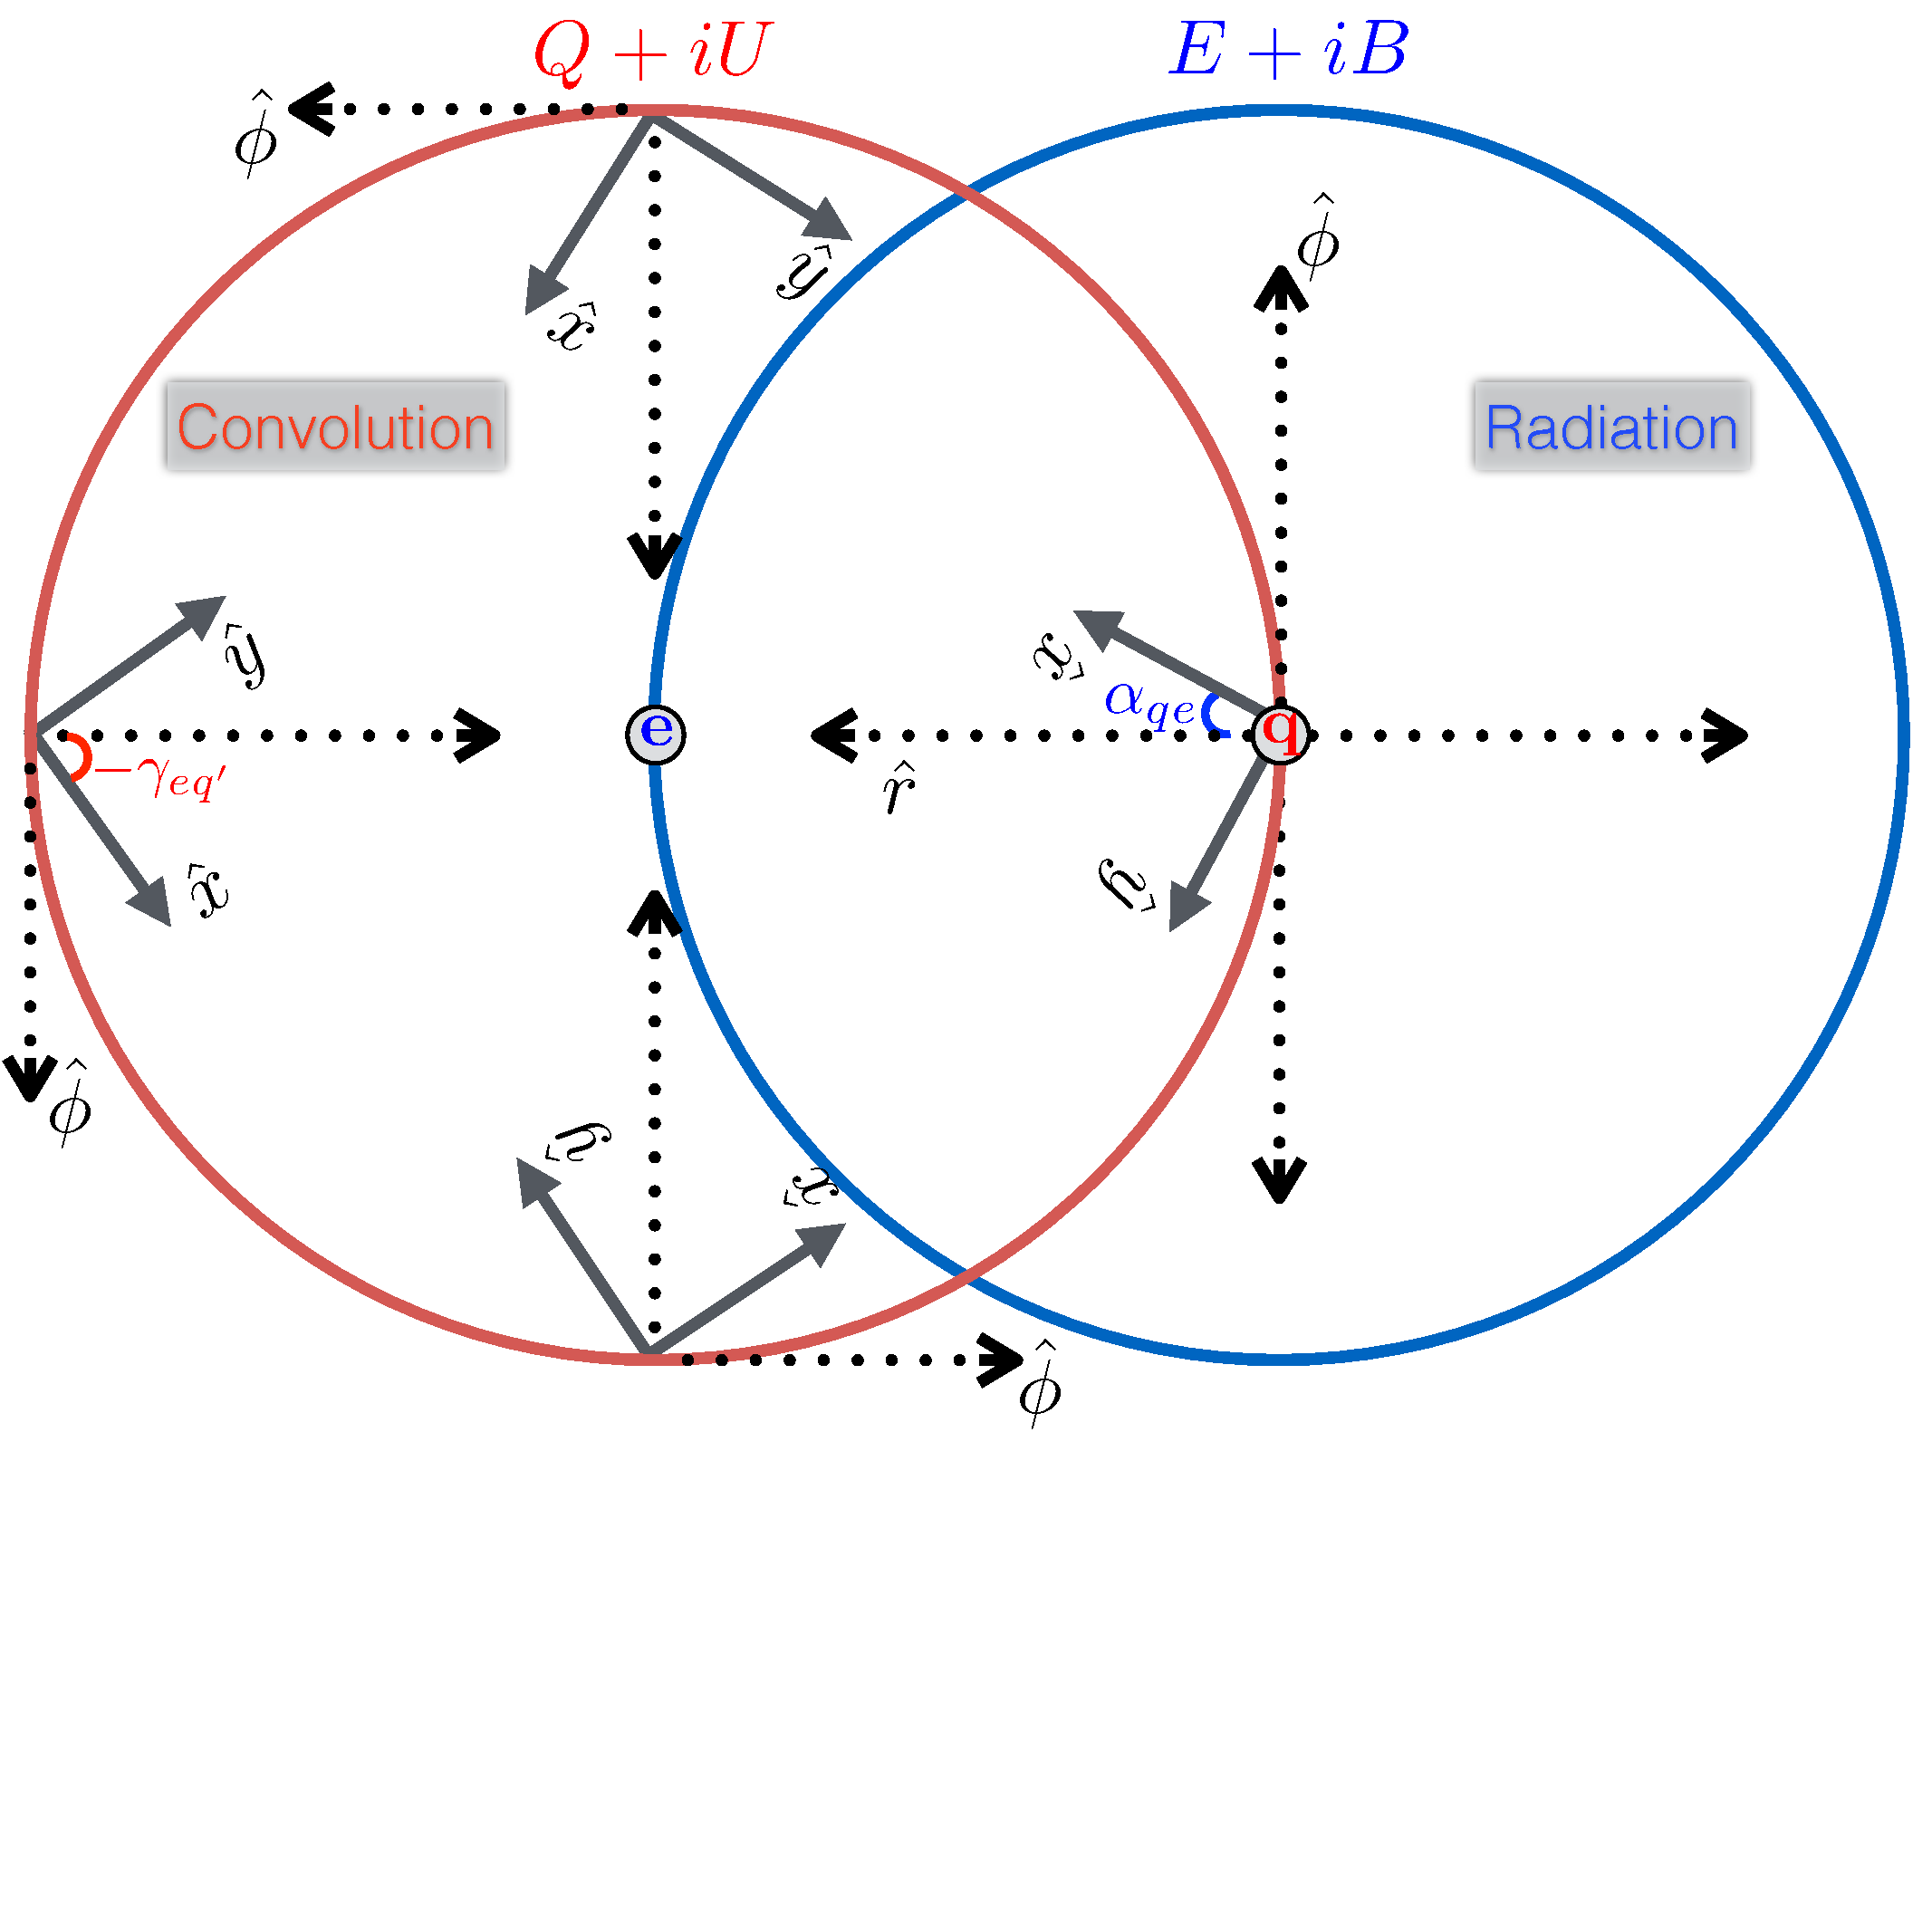
\includegraphics[width=0.5\columnwidth]{radiation_convolution.pdf}
\caption{}
\label{fig:euler_angles}
\end{figure}
%
\textit{Radiating:} On the contrary, while working from the frame of the pixel ``q'', the Euler angles to the surrounding pixels are: $\alpha_{qe}, \beta_{qe},\gamma_{qe}$. The E \& B mode maps resulting from the Stokes Q \& U parameters specified at the location $\hat{n}_q$ is given by the following expression,
%
\beq  \label{eq:qu2eb_radiation_explicit}
\bmat E_e \\ B_e  \emat_{q} =- {{}_{\mm}f}(\beta_{qe},\ell_{\rm min},\ell_{\rm max})\bmat \cos(2 \alpha_{q e}) & \sin(2\alpha_{q e})\\  -\sin(2 \alpha_{q e})  & \cos(2 \alpha_{q e}) \emat  \bmat Q_{q} \\ U_{q}  \emat \Delta \Omega \,.
\eeq
%
The total map of E \& B modes can be simply evaluated by summing over the contribution from the Stokes parameters at each location $\hat{n}_q$ : $\bar{S} = \sum_{q=1}^{N_{\rm pix}} \bar{S}_q$. The above expression can again be cast in a more concise form as follows,
%
\begin{subequations} \label{eq:qu2eb_radiation_concise}
\beqry 
\left[E + iB\right] &=& -\Delta \Omega  \sum_{q=1}^{N_{\rm pix}} \Big[ {}_{+2}X(\hat{n}_{q}) e^{-i2\alpha_{q e}} \Big]  {{}_{\mm}f}(\beta_{q e}) \,, \\
&=&    \sum_{q=1}^{N_{\rm pix}} \Bigg\lbrace {}_{+2}X(\hat{n}_{q}) \cdot \left[ - \Delta \Omega \sum_{\ell=\ell_{\rm min}}^{\ell_{\rm max}} \sqrt{\frac{2 \ell+1}{4 \pi}}Y^*_{\ell 2}(\beta_{qe},\alpha_{qe}) \right] \Bigg\rbrace \,, \\
&=& \sum_{q=1}^{N_{\rm pix}} {}_{+2}X(\hat{n}_{q}) \cdot  \mathcal{M}_{Green}(\hat{n}_{q}) \,,
\eeqry
\end{subequations}
%
where ``$\cdot$'' denotes a simple scalar multiplication. \revisit{$\mathcal{M}_{Green}(\hat{n}_{q})$ is response of the real space operator $\bar{O}$ when operated on a Stokes field: $\delta(\hat{n}-\hat{n}_q) + i \delta(\hat{n}-\hat{n}_q)$, hence it can be thought of as the Green's function of the real space operator.} \comment{Is this interpretation correct ? Is the complex delta function a spin 2 function ?}

Recall that the product of two functions with spins $s_1$ and $s_2$ results in a function with spin $s_1 + s_2$: ${}_{s_1 +s_2}f = {}_{s_1}g \,{}_{s_2}h$ \comment{The following argument is that of the product of a number with a field, so is this relevant ?}. If one rotates the cartesian coordinates in the tangent plane at location $\hat{n}_q$ by an angle $\phi$ about the local $\hat{z}_q$ axis, the Stokes parameters in the new rotated frame are given by: ${}_{+2}X(\hat{n}_q) \xrightarrow{\mathcal{R}_{\hat{z}_q}(\phi)} {}_{+2}X(\hat{n}_q) e^{-i2\phi} $. \revisit{Recall that the Euler angle $\alpha_{qe}$ in the $z-y_1-z_2$ sense of rotations is such that it aligns the local $\hat{x}_q$-axis along the geodesic in the direction of $\hat{n}_e$. Now if the local planar axes are already rotated by an angle $\phi$ then $\alpha_{qe} \rightarrow \alpha_{qe} - \phi$ and therefore one can see that: $e^{-i2\alpha_{qe}} \xrightarrow{\mathcal{R}_{\hat{z}_q}(\phi)} e^{-i2\alpha_{qe}} e^{i2\phi}$.} The Euler angles $|\beta_{qe}|$ which measure the angular distance between pixels remains unaltered under this local rotation operation.  Given these transformation properties one can now note that the product ${}_{+2}X(\hat{n}_q)e^{-i2\alpha_{qe}}$ is invariant under rotations  $\mathcal{R}_{\hat{z}_q}(\phi)$ and hence must form a spin-0 field.  This argument makes intuitive, the construction of the spin-0 E and B modes of polarization from the measured Stokes parameters. \revisit{Here it is also interesting to note that the E-modes are constructed by product of functions $(U\sin{2 \alpha}, Q\cos{2\alpha})$ which have the same parity and hence have even parity while the B-modes are constructed by multiplying functions $(Q\sin{2 \alpha}, U\cos{2\alpha})$ of opposite parity and hence have an odd parity.}

Using \eq{eq:qu2eb_radiation_explicit} one can see that when $q=e ~(\beta_{qq}=0\,,\, \alpha_{qq}=0,2\pi,4\pi,...)$: $E_q=-{{}_{\mm}f}(\beta_{qq})Q_q$ and $B_q = -{{}_{\mm}f}(\beta_{qq})U_q$ which does not transform as a spin-0 field under local rotations unless ${{}_{\mm}f}(\beta_{qq}=0)=0$. One can make a similar argument when pixels ``q'' and ``e'' are diametrically opposite. Therefore the radial kernels have to satisfy the constraint that they vanish at $\beta = 0, \pi$. The radial kernel ${{}_{\mm}f}(\beta)$ is constructed by forming a weighted linear combination of $P_{\ell}^2$ Legendre polynomials which have the following limiting form: $P_{\ell}^2(\beta) \propto \sin^2{\beta} \rightarrow 0 $ as $\beta \rightarrow 0 ,\pi$ and therefore satisfy this necessary constraint. 

The real space operator has a azimuthal part which depends only on the Euler angle $\alpha_{qe} (\gamma_{eq})$, has no multipole $\ell$ dependence and is the crucial operation which translates between the two different spin representation of CMB polarization. The radial part of the kernel is specified by the function ${}_{\mm}f(\beta,\ell_{\rm min},\ell_{\rm max})$, it depends only on the angular separation $|\beta_{eq}|$ between pixels and completely incorporates the multipole $\ell$ dependence of the kernel. It's the radial part of the kernel that determines the locality of the real space operator.
%--------------------------------------------------------
%--------------------------------------------------------
\subsection{Evaluating Stokes parameters $Q$ \& $U$ from scalar fields $E$ \& $B$}\label{sec:eb2qu}
The real space operator which translates $E$ \& $B$ fields to Stokes parameters $Q$ \& $U$ can be derived using a similar procedure. The inverse operator is given by the following expression,
%
\begin{subequations}
\beqry
\bar{P} &=& \bar{T}^{-1} *{{}_2\mathcal{Y}} *\tilde T *{{}_0\mathcal{Y}^{\dagger}}\bar{S} = \frac{1}{2} \bar{T}^{\dagger} *{{}_2\mathcal{Y}} *\tilde T *{{}_0\mathcal{Y}^{\dagger}}\bar{S} \,,  \\
&=&  \bar O^{-1} *\bar{S}\,.
\eeqry
\end{subequations}
%
Providing the explicit derivation here will be redundant with that described in the previous sections and hence we avoid that. The inverse operator $\bar{O}^{-1}$ can be derived by realizing that $\mm^{-1}$ is given by the following expression,
%
\beq
\mm^{-1} = \sum_{\ell m}  {{}_{2}}Y_{\ell m}(\hat n_q) {}_{0}Y^*_{\ell m}(\hat n_e) \, 
\eeq
%

 The inverse operator is given by the following expression,
%
\beq
{\bar O}^{-1}=-\bmat \mathcal{M}_{r} & -\mathcal{M}_{i} \\  \mathcal{M}_{i}  & \mathcal{M}_{r} \emat_{2 N_{\rm pix} \times 2 N_{pix}} =-{{}_{\mm}f}(\beta_{eq},\ell_{\rm min},\ell_{\rm max})\bmat \cos(2 \alpha_{eq}) & -\sin(2\alpha_{eq})\\  \sin(2 \alpha_{eq})  & \cos(2 \alpha_{eq}) \emat \,.
\eeq
%
where all the symbols have the same meaning as discussed in \sec{sec:qu2eb}. Note that the kernel in the above equation differs from the one in \eq{eq:op_qu2eb} by a change in sign on the off-diagonals of the block matrix and the pixel indexing is reversed $ e \leftrightarrow q$. We can evaluate the Stokes parameters  $Q$ \& $U$ from the scalar fields $E$ \& $B$ by evaluating the following expression,
%
\beq \label{eq:eb2qu_convolution_explicit}
\bmat Q_i \\ U_i  \emat=-\Delta \Omega\sum_{j=1}^{N_{\rm pix}} {{}_{\mm}f}(\beta_{ij},\ell_{\rm min},\ell_{\rm max})\bmat \cos(2 \alpha_{ij}) & -\sin(2\alpha_{ij})\\  \sin(2 \alpha_{ij})  & \cos(2 \alpha_{ij}) \emat  \bmat E_j \\ B_j  \emat \,,
\eeq
%
where all the symbols have their usual meaning. The above equation can again be expressed more concisely as follows,
%
\begin{subequations} \label{eq:eb2qu_simple}
\beqry 
{}_{+2}\bar{X}(\hat{n}_0) &=& - \Delta \Omega \sum_{j=1}^{N_{\rm pix}} \left(\sum_{\ell=\ell_{\rm min}}^{\ell_{\rm max}} \frac{2 \ell+1}{4 \pi} \sqrt{\frac{(\ell-2)!}{(\ell+2)!}}  P_{\ell}^{2}(\beta_{0j}) \right)  {\Bigg( e^{i2 \alpha_{0j}}   [E+iB](\hat{n}_j) \Bigg)} \,, \label{eq:eb2qu_physical}\\
&=& - \Bigg\lbrace \left[ \sum_{\ell=\ell_{\rm min}}^{\ell_{\rm max}} \sqrt{\frac{2 \ell+1}{4 \pi}}Y_{\ell 2} \right]  \circ [E+iB]  \Bigg\rbrace (\hat{n}_0) \,, \\
&=& - \Bigg\lbrace \mathcal{M} \circ [E + iB] \Bigg\rbrace(\hat{n}_0)\,, 
\eeqry
\end{subequations}
%
which $\circ$ is to be interpreted as a convolution. The only change in the convolution kernel as compared to that in \eq{eq:qu2eb_simple} is that the $Y_{\ell 2}$ functions are not conjugated. This can again be simply understood as the construction of a spin-2 field by taking a product of a spin-0 field $[E +iB]$ with a spin $+2$ field $e^{+i2\alpha}$. The radial dependence of the operator ${\bar O}^{-1}$  is identical to the that of ${\bar O}$ as one may have expected. From the perspective of the scalar field $[E + iB]$, all the coordinate dependence of the Stokes parameters is encoded in the function $e^{+i2\alpha}$.  The radial functions again have to vanish at $\beta \rightarrow 0,\pi$ for the same reasons that the function $e^{+i2\alpha}$ is ill defined at these locations.
%--------------------------------------------------------
%--------------------------------------------------------
\subsection{Decomposing Stokes parameters $Q$ \& $U$  into those corresponding to $E$ \& $B$ modes respectively}
We can only measure the total Stokes vector which is a sum of the Stokes vectors corresponding to the respective scalar modes. The $E$ \& $B$ modes are orthogonal to each other, in the sense that their respective operators are orthogonal to each other as seen in \eq{eq:op_eb_ortho}. It is possible to decompose the Stokes vector \vp{} into one \vp{\rm E} that purely contributes to $E$ modes and another \vp{\rm B} that purely contribute to the $B$ modes of polarization. In this section we derive the real space operators which operate on the total Stokes vector and yield this decomposition, without ever having to explicitly evaluate the scalar modes. Though the algebra is a little more involved, the derivation is similar to that discussed in \sec{sec:qu2eb}, hence we refrain from presenting the detailed calculations here, but outline the key points. We use the harmonic space projection operators $\tilde O_{E/B}$, defined in \eq{eq:har_eb_op}, to derive the respective real space operators. The Stokes parameters corresponding to each scalar mode are given by the following expressions,
%
\beqry
\bar{P}_E &=&  [\bar T^{-1} * {{}_2\mathcal{Y}} *\tilde T * \tilde O_E* \tilde T^{-1}* {{}_2\mathcal{Y}^{\dagger}} *\bar T] *\bar{P}  \,, \\
&=& [\frac{1}{4} \bar T^{\dagger } * {{}_2\mathcal{Y}} *\tilde T * \tilde O_E* \tilde T^{\dagger} * {{}_2\mathcal{Y}^{\dagger}} *\bar T ]*\bar{P}  \,, \nonumber \\
&=&  \bar O_{E}*\bar{P} \,,\nonumber \\
\bar{P}_B &=&  [\bar T^{-1}* {{}_2\mathcal{Y}}* \tilde T* \tilde O_B* \tilde T^{-1}* {{}_2\mathcal{Y}^{\dagger}}* \bar T]*\bar{P}  \,, \\
&=& [\frac{1}{4} \bar T^{\dagger } * {{}_2\mathcal{Y}} *\tilde T * \tilde O_B* \tilde T^{\dagger} *{{}_2\mathcal{Y}^{\dagger}} *\bar T] *\bar{P}   \,, \nonumber\\
&=&  \bar O_{B}*\bar{P} \,. \nonumber
\eeqry
%
We contract over all the matrix operators to arrive at the the real space operators. On working through the algebra it can be shown that the real space operators have the following form,
%
\beq
\bar O_{E/B} = 0.5 \bmat \mathcal{I}_{r} & \mathcal{I}_{i} \\  -\mathcal{I}_{i}  & \mathcal{I}_{r} \emat \pm \bmat \mathcal{D}_{r} & \mathcal{D}_{i} \\  \mathcal{D}_{i}  & - \mathcal{D}_{r} \emat \,,\\
\eeq
where $\mathcal{I}_{r} ~\&~ \mathcal{D}_{r}$ and $\mathcal{I}_{i} ~\&~ \mathcal{D}_{i}$ are the real and complex parts of the following complex functions,
%
\begin{subequations}
\beqry
\mathcal{I} &=& \mathcal{I}_{r} + i \mathcal{I}_{i} = \sum_{\ell m} {_{-2}Y}_{\ell m}(\hat n_i) {_{-2}Y}^*_{\ell m}(\hat n_j) \,, \\
\mathcal{D}  &=& \mathcal{D}_{r} + i\mathcal{D}_{i} = \sum_{\ell m} {_2Y}_{\ell m}(\hat n_i) {_{-2}Y}^*_{\ell m}(\hat n_j) \,.
\eeqry
\end{subequations}
%
These functions can be further simplified using the identity of spin spherical harmonics given in \eq{eq:sum_spin_shf}. Specifically it can be shown that these functions reduce to the following mathematical forms,
%
\beqrys \label{eq:fn_i}
\mathcal{I}(\hat{n}_i, \hat{n}_j) &=& \sum_{\ell} \sqrt{\frac{2\ell+1}{ 4 \pi}}{_{-2}Y}_{\ell2}(\beta_{ij}, \alpha_{ij}) ~ \rm{e}^{i2 \gamma_{ij}} \label{eq:healpix-compatible-i} = \mathcal{I}_r + i \mathcal{I}_i \,, \\
\mathcal{I}_r + i \mathcal{I}_i &=& \Big [ \cos(2 \alpha_{ij} +  2\gamma_{ij}) + i \sin(2 \alpha_{ij} +  2 \gamma_{ij}) \Big]   {{}_{\mi}f}(\beta_{ij},\ell_{\rm min},\ell_{\rm max}) \,,
\eeqrys
%
%
\beqrys \label{eq:fn_d}
\mathcal{D}(\hat{n}_i, \hat{n}_j) &=& \sum_{\ell} \sqrt{\frac{2\ell+1}{ 4 \pi}}{_2Y}_{\ell 2}(\beta_{ij}, \alpha_{ij}) ~ \rm{e}^{- i2 \gamma_{ij}} \label{eq:healpix-compatible-m} =\mathcal{D}_r + i \mathcal{D}_i \,, \\
\mathcal{D}_r + i \mathcal{D}_i &=&  \Big [ \cos(2 \alpha_{ij} - 2\gamma_{ij}) + i \sin(2 \alpha_{ij} -  2 \gamma_{ij}) \Big]   {{}_{\md}f}(\beta_{ij},\ell_{\rm min},\ell_{\rm max}) \,,
\eeqrys
%
where the radial functions are given by,
%
\beq
{{}_{\mdi}f}(\beta,\ell_{\rm min},\ell_{\rm max}) = \sum_{\ell=\ell_{\rm min}}^{\ell_{\rm max}} \sqrt{\frac{2\ell+1}{ 4 \pi}} {{}_{ \mdi}f}_{\ell}(\beta) \label{eq:f2_rad_ker}\,,
\eeq
%
where the functions ${{}_{ \pm 2}f}_{\ell}(\beta)$ are expressed in terms of $P_{\ell}^2$ Legendre polynomials and are given by the following explicit mathematical forms,
 %
 \beqry
 _{\mdi}f_{\ell}(\beta) &=& 2 \frac{(\ell-2)!}{(\ell+2)!}  \sqrt{\frac{2\ell +1 }{4 \pi}} \Bigg[ - P_{\ell}^{2} (\cos  \beta) \left( \frac{\ell-4}{\sin^2 \beta} + \frac{1}{2}\ell(\ell-1) \pm \frac{2 (\ell-1) \cos \beta}{\sin^2 \beta} \right) \nonumber \\ 
&+& P_{\ell-1}^2 (\cos \beta) \left( (\ell+2) \frac{\cos \beta}{\sin^2 \beta} \pm \frac{2 (\ell+2)}{ \sin^2 \beta } \right) \Bigg] \,. \label{eq:rad_ker_quequbqu}
 \eeqry
 %
Finally the Stokes parameters corresponding to the respective scalar fields can be computed by evaluating the following expressions, 
 %
\beqry \label{eq:op_qu2equbqu}
\bmat Q_i \\ U_i  \emat_{E/B} &=& \sum_{j=1}^{N_{\rm pix}} \Bigg\lbrace {{}_{\mi}f}(\beta_{ij},\ell_{\rm min},\ell_{\rm max}) \bmat \cos(2 \alpha_{ij} + 2\gamma_{ij}) & \sin(2\alpha_{ij} +2 \gamma_{ij}) \\  -\sin(2\alpha_{ij} +2 \gamma_{ij})  & \cos(2 \alpha_{ij} + 2 \gamma_{ij}) \emat  \bmat Q_j \\ U_j  \emat  \\ &\pm& {}_{\md}f(\beta_{ij},\ell_{\rm min},\ell_{\rm max}) \bmat \cos(2 \alpha_{ij} - 2\gamma_{ij}) &  \sin(2\alpha_{ij} - 2 \gamma_{ij}) \\  \sin(2\alpha_{ij} - 2 \gamma_{ij})  & - \cos(2 \alpha_{ij} - 2 \gamma_{ij}) \emat  \bmat Q_j \\ U_j  \emat \Bigg\rbrace 0.5 \Delta\Omega  \,, \nonumber 
\eeqry
%
where all the symbols have their usual meaning. The above expression can be cast in the further simplified form,
%
\begin{subequations}
\beqry
{}_{+2}X_{E/B} &=&0.5 \Delta \Omega\sum_{j=1}^{N_{\rm pix}}  {{}_{\mi}f}(\beta_{ij}) e^{-i2 (\alpha_{ij} + \gamma_{ij})} {}_{+2}X_j \pm {{}_{\md}f}(\beta_{ij}) e^{i2 (\alpha_{ij} - \gamma_{ij})} {}_{+2}X_j^*\,, \label{eq:qu2equbqu_explicit_convolution} \\
&=& 0.5 \Bigg\lbrace \mathcal{I}^* \circ {}_{+2}X\pm \mathcal{D} \circ {}_{+2}X^* \Bigg\rbrace \,, \label{eq:qu2equbqu_convolution}
\eeqry
\end{subequations}
%
where in \eq{eq:qu2equbqu_explicit_convolution} we have suppressed the explicit multipole dependence of functions $_{\pm 2}f$ for brevity and in \eq{eq:qu2equbqu_convolution} $\circ$ denotes a convolution. \comment{Here it will be nice to interpret $e^{i2\gamma}[E-iB]$. We don't understand this as of now.}

\comment{Recheck the math described below}
The function $\mathcal{I}$ is a band limited version of the delta function ($\lim_{\ell \rightarrow \infty} \mathcal{I} = \delta(\hat{n}_i - \hat{n}_j)$). When interpreted as a matrix it is a band limited version of the identity matrix. Though it has non vanishing off diagonal elements ($\mathcal{I} \neq 0 $ when $\hat{n}_i \neq \hat{n}_j$) owing to the band limit, for all practical purposes $\mathcal{I}$ acts like an identity operator as is confirmed by the following set of identities: (i) $\mathcal{I}*\mathcal{I}=\mathcal{I}$ ; (ii) $\mathcal{D}*\mathcal{I}=\mathcal{D}$. Also $\mathcal{D}^*$ is the inverse of $\mathcal{D}$ in this band limited sense: $\mathcal{D}^**\mathcal{D}=\mathcal{I}$. It is useful to note that the operator $\mathcal{D}$ is a complex but symmetric matrix and $\mathcal{I}$ is an Hermitian operator. Using these properties of the operators $\mathcal{I}$ and $\mathcal{D}$, one can verify that the real space operators satisfy the following identities,
%
\begin{subequations}
\beqry
\bar O_E * \bar O_E &=& \bar O_E ~~;~~ \bar O_B * \bar O_B = \bar O_B \,, \\
\bar O_E*\bar O_B &=& 0 \,,\\
\bar O_E + \bar O_B &=& \mathcal{I} \,,
\eeqry
\end{subequations}
%
which are the real space analogues of \eq{eq:har_op_prop}. While testing the above stated identities one encounters terms like $\mathcal{D}*\mathcal{I}^*,\mathcal{I}^**\mathcal{I} \textrm{ and }  \mathcal{I}*\mathcal{I}^*$ which cannot be simply interpreted, but they always occur in pairs with opposite signs, hence exactly canceling each other. 

Note that unlike in the harmonic case, the sum of the operators is not exactly an identity matrix. 
%\comment{Isn't it possible to do some real space operations which doesn't care for the band limit but still returns the required decomposition into the respective scalar modes ?} 
This non-exactness is representative of the loss of information resulting from making this transformation on the measured data with some imposed band limit. Forcing the sum of the operators to be exactly an identity matrix compromises the orthogonality property of the $\bar{O}_E$ \& $\bar{O}_B$ operators, which is exact.